\chapter{Previous Work}\label{chapt:previous}
\textit{The idea of using satellite data has been researched within many communities. Several automated and semi-automated ways are proposed to tackle the problem of detecting roads. These ways are quite different due to the different strategies and algorithms used by them. The different strategies come into the picture to tackle the various challenged like noisy data, occlusions, distortion and complex backgrounds which appears in images.}

\section{Road detection}
The journey to digitally identify the roads started with the topic of reducing cost and increasing productivity. One of the first road detection algorithms were static methods and focused on the color and geometry of roads. This was quite unreliable as shadows on roads had a similar color range, this resulted in many errors and discontinuities~\cite{Detecting_interections_using_color,Detecting_roads_using_color}. Another disadvantage was the need for high-resolution images (Almost 0.2~m~-~0.5~m), which is hard to get. The idea was then improvised to include texture cues for road detection~\cite{using_texture_for_road_detection,baumgartner1999automatic}. The accuracy was indeed better, but the need for a very high-resolution image remained a problem. With the Machine learning techniques, the pixel-level classification started to give improved performance~\cite{road_detection_using_neural_nets_SVM,road_detection_using_env_learning,road_detection_using_SVM_online_learning}.

The Support Vector Machine~(SVM) methods have a good generalization ability and thus widely used in object detection from a given image. They are, at most times, more accurate and give consistent robust results than other classification techniques such as K-nearest neighbor. Nevertheless, the estimation of kernel functions and the choice of the dimensional space and training samples led to the SVM classifier~\cite{YagerSowmya2003,melgani2004classification}. This was done using edge-based features such as gradient, intensity, edge length, and classified objects in a high-resolution image. SVM approaches are well suited for multispectral data where we have an adequate number of vectors to classify objects~\cite{Simler2011}.

In 2003, Tu-Ko presented a robust approach, in which a back-propagation~(BP) neural network was trained with the spectral and edge information to find the road centerline. Although errors prop in, the model was still useful as a whole. Disadvantages of BP neural network include slow convergence speed, the need for an extensive training data set, inability to find global minima, and over-fitting risks. Since then, many types of neural networks like fuzzy neural networks~\cite{mokhtarzade2008automatic} and Convolutional Neural Networks~(CNN) have been used to capture the spacial contexts of road networks, giving much better accuracies on fewer resources.

With the developments of GPUs and the progress of ResNet architectures, even Deep Convolutional Neural Networks~(DCNN) have been researched and changed the way road extraction works. The recent developments with encoder-decoders, dilations, and fuzzy logic have inspired state-of-the-art algorithms like UNet, SegNet, LinkNet, and its further improvements like D-LinkNet and AD-LinkNet~(Figure~\ref{fig:compare_road}). Moreover, competitions pitch in the researchers by providing them with a precise dataset and motivating them to thrive and excel in the world race.

\begin{figure}[h!]
  \centering
  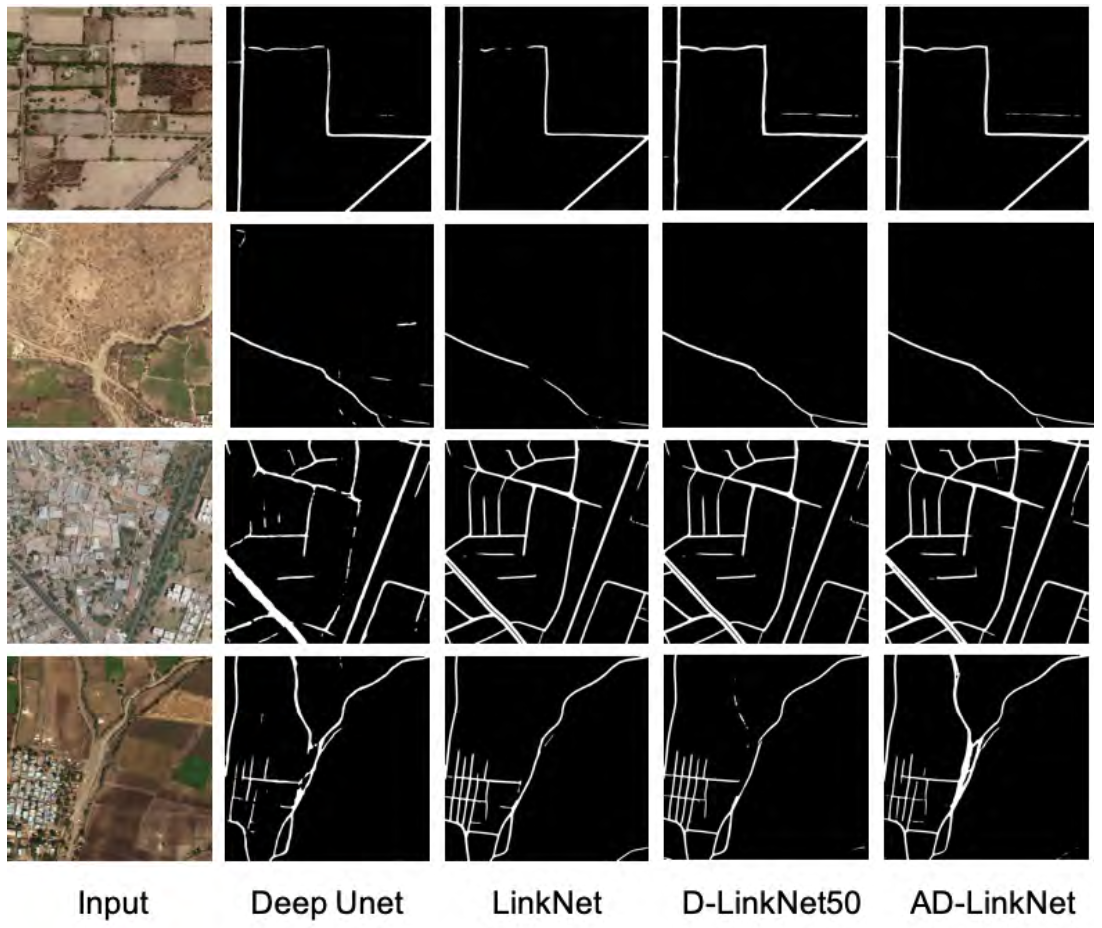
\includegraphics[width=\textwidth]{compare_road}
  \caption[Comparison of different Road-detection models.]{Comparison of different Road-detection models. Adapted from~\cite{AD-LinkNet}}
  \label{fig:compare_road}
\end{figure}


\section{Super-resolution}
Many models have proposed methods to obtain a super-resolution image from the given image. Most of the techniques use bicubic upsampling of the image as an input to the proposed neural network model. However, this was inefficient as a significant part of memory is required for performing bicubic upsampling. The authors of~\cite{EDSR} additionally questioned the architectural optimality used in the existing networks. Though neural networks provide significantly improved performance in terms of peak signal-to-noise ratio (PSNR) in the SR problem, it is also proven to be quite sensitive to minor architectural changes. The outputs differ in performance with different training techniques. The authors further proposed an enhanced deep super-resolution network (EDSR) with performance exceeding the past state-of-the-art super-resolution models. This was achieved by carefully designing model architecture using sophisticated optimization methods in training the neural networks.

Secondly, the authors noticed that most existing models treat the super-resolution of different scale factors as an independent problem. There is no consideration of learning the mutual relationship between different scales. With efforts such as the development of VSDR, this relationship is proved to be feasible and much more accurate than the single-scale models, though at the cost of heavier computation time and memory utilization. Further work was restricted by a lack of ability to use very deep neural networks.

With the break-through changes brought by concepts of skip-connects and residual blocks, neural networks were shown to be trained with 100+ layers. SRNet solved incorporated the ResNet architecture and solved the problem of high memory utilization. Because ResNet architecture was proposed to solve higher-level computer vision problems such as image classification and detection, its use directly for a low-level problem like computer vision can be optimized.

EDSR proposes using a modified type of residual block to remove the unnecessary elements and optimize the model's performance. Secondly, a new architecture is used with fewer parameters but showing comparable performance. The Figure~\ref{fig:compare_SR} shows a comparison between different SR algorithms.

\begin{figure}[h!]
  \centering
  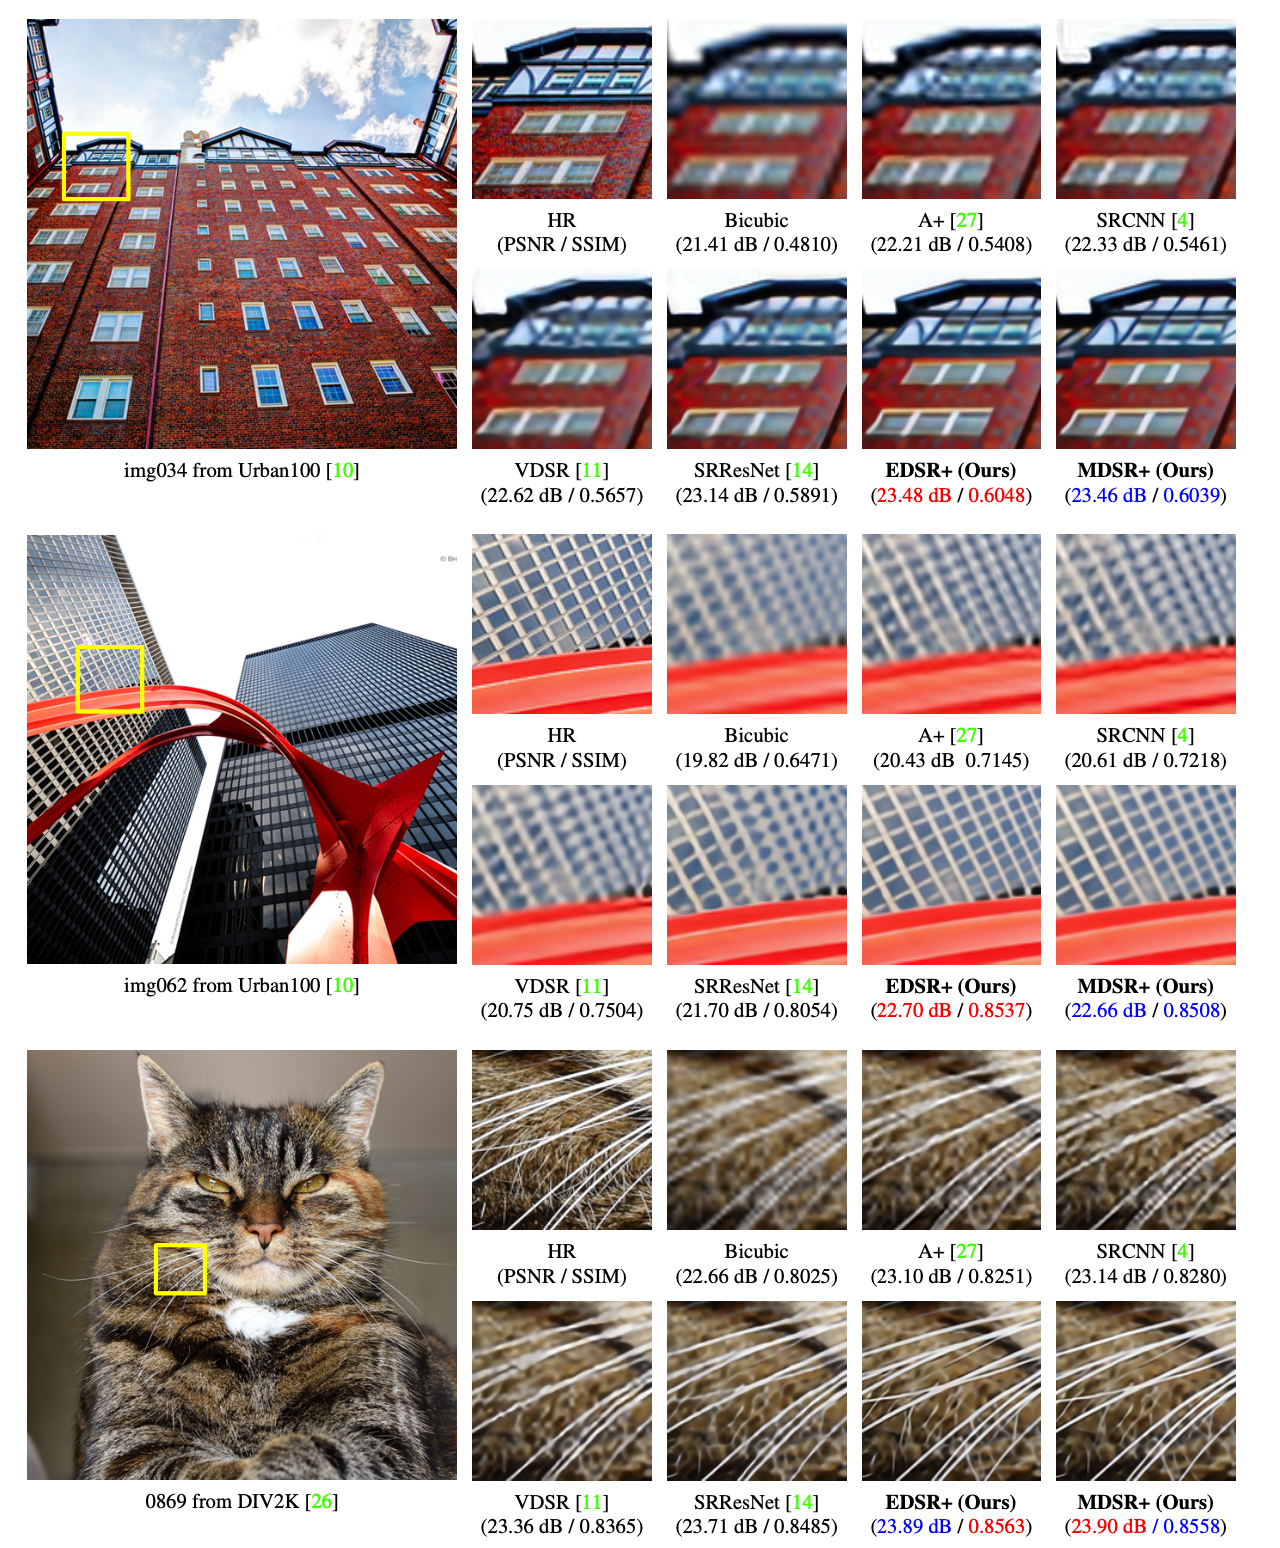
\includegraphics[width=\textwidth]{compare_SR}
  \caption[Comparison of different Super-resolution models.]{Comparison of different Super-resolution models. HR is raw high resolution image taken. Adapted from~\cite{EDSR}}
  \label{fig:compare_SR}
\end{figure}
